\documentclass{article}

% Language setting
\usepackage[english]{babel}

% Set page size and margins
% Replace `letterpaper' with `a4paper' for UK/EU standard size
\usepackage[letterpaper,top=2cm,bottom=2cm,left=3cm,right=3cm,marginparwidth=1.75cm]{geometry}

% Useful packages
\usepackage{amsmath}
% --- Code listings ---
\usepackage{listings}
\usepackage{xcolor}
\definecolor{codegreen}{rgb}{0,0.6,0}
\definecolor{codegray}{rgb}{0.5,0.5,0.5}
\definecolor{codepurple}{rgb}{0.58,0,0.82}
\definecolor{backcolour}{rgb}{0.95,0.95,0.92}

\lstdefinestyle{mystyle}{
    backgroundcolor=\color{backcolour},   
    commentstyle=\color{codegreen},
    keywordstyle=\color{magenta},
    numberstyle=\tiny\color{codegray},
    stringstyle=\color{codepurple},
    basicstyle=\ttfamily\footnotesize,
    breakatwhitespace=false,         
    breaklines=true,                 
    captionpos=b,                    
    keepspaces=true,                 
    numbers=left,                    
    numbersep=5pt,                  
    showspaces=false,                
    showstringspaces=false,
    showtabs=false,                  
    tabsize=2
}

\lstset{style=mystyle}
% --- End Code Listings
\usepackage{graphicx}
\usepackage{float}
\usepackage{caption}
\captionsetup{labelformat=empty} 
% \usepackage{subcaption}
\usepackage[colorlinks=true, allcolors=blue]{hyperref}
\graphicspath{{./figures/}}

\title{ECE 637 - Lab 4}
\author{Colin Braun}

\begin{document}
\maketitle

\section{Histogram of an Image}
\begin{figure}[H]
    \centering
    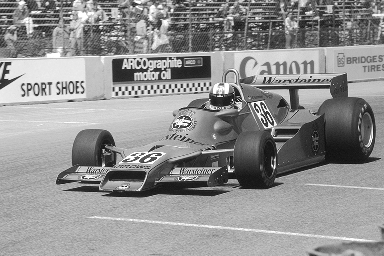
\includegraphics[width=1\textwidth]{../race.png}
    \caption{race.tif image}
\end{figure}
\begin{figure}[H]
    \centering
    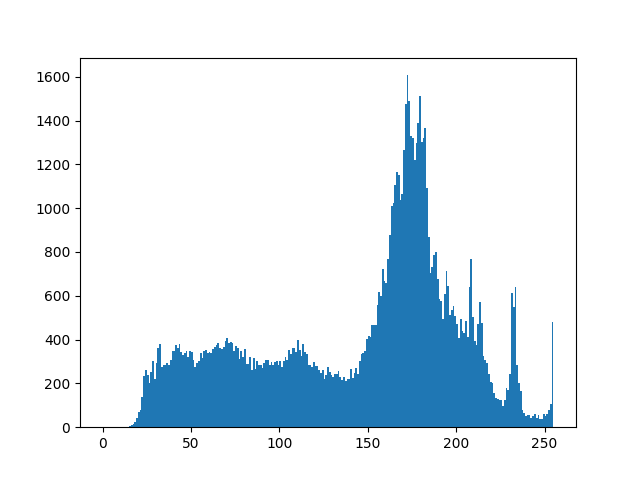
\includegraphics[width=1\textwidth]{../race-histogram.png}
    \caption{Histogram of race}
\end{figure}
\begin{figure}[H]
    \centering
    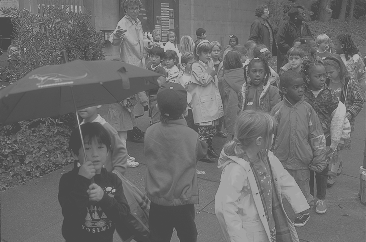
\includegraphics[width=1\textwidth]{../kids.png}
    \caption{kids.tif image}
\end{figure}
\begin{figure}[H]
    \centering
    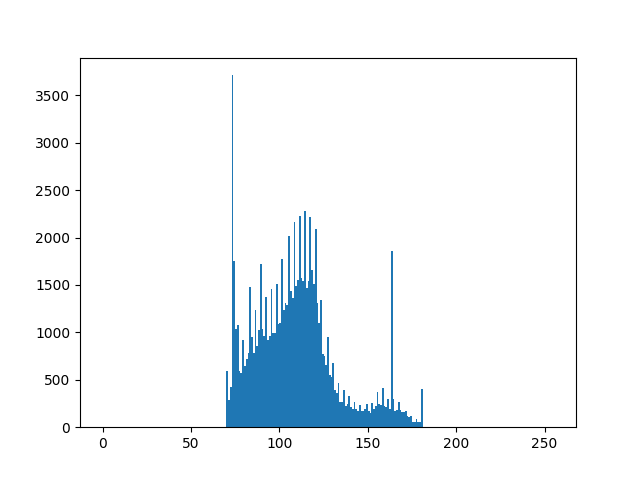
\includegraphics[width=1\textwidth]{../kids-histogram.png}
    \caption{Histogram of kids.tif}
\end{figure}



\section{Histogram Equalization}
\subsection{Function equalize}
\lstinputlisting[language=Python, firstline=6, lastline=20]{../section2.py}
\subsection{Plot of $\hat{F}_x(i)$ for kids.tif}
\begin{figure}[H]
    \centering
    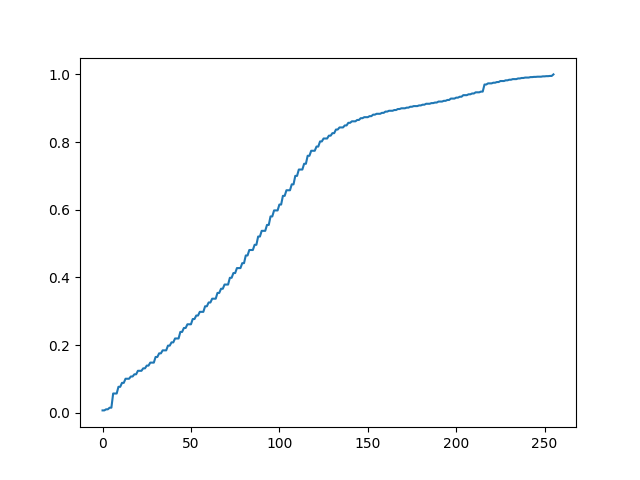
\includegraphics[width=1\textwidth]{../kids-fx.png}
    \caption{$\hat{F}_x(i)$}
\end{figure}
\subsection{Plot of equalized image's histogram}
\begin{figure}[H]
    \centering
    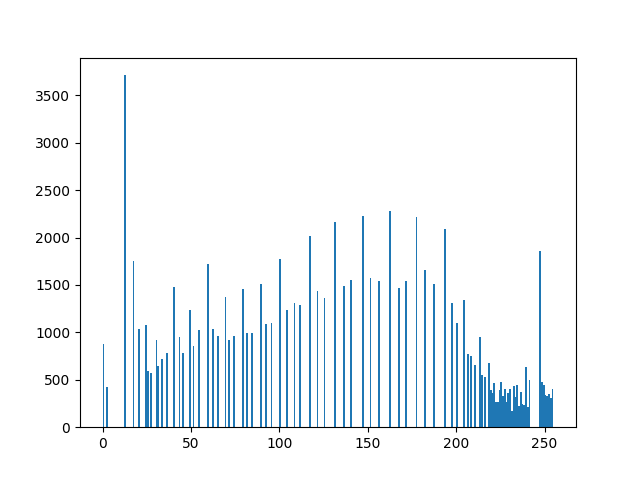
\includegraphics[width=1\textwidth]{../kids-equalized-histogram.png}
    \caption{Equaliazed image's histogram}
\end{figure}
\subsection{Plot of equalized image}
\begin{figure}[H]
    \centering
    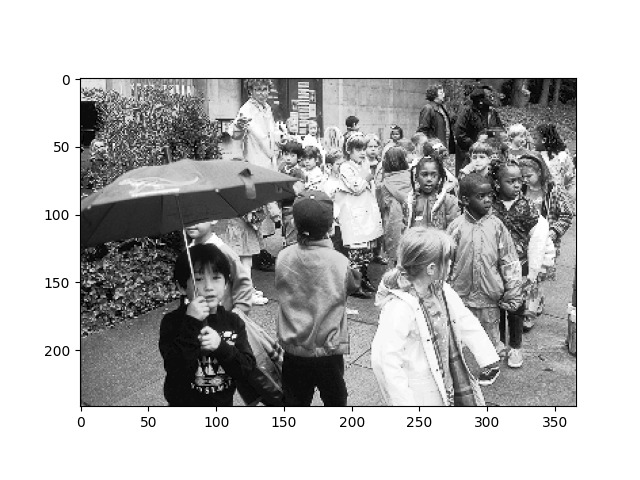
\includegraphics[width=1\textwidth]{../kids-equalized-image.png}
    \caption{Equalized image}
\end{figure}



\section{Contrast Stretching}
\subsection{Code for stretch}
\lstinputlisting[language=Python, firstline=6, lastline=22]{../section3.py}
\subsection{Transformed image and its histogram}
\begin{figure}[H]
    \centering
    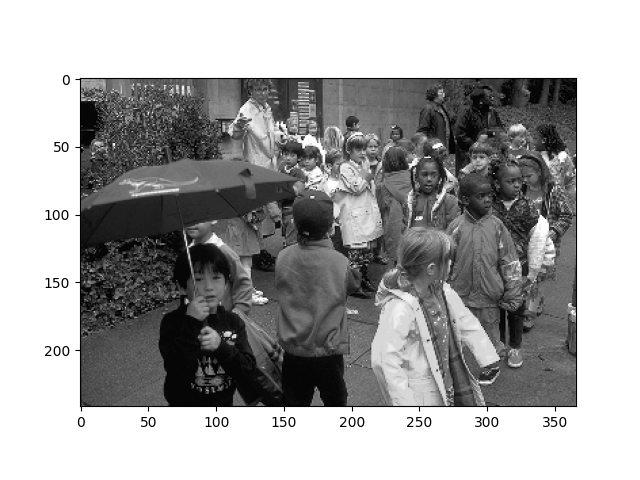
\includegraphics[width=1\textwidth]{../kids-stretched.png}
    \caption{Stretched image}
\end{figure}
\begin{figure}[H]
    \centering
    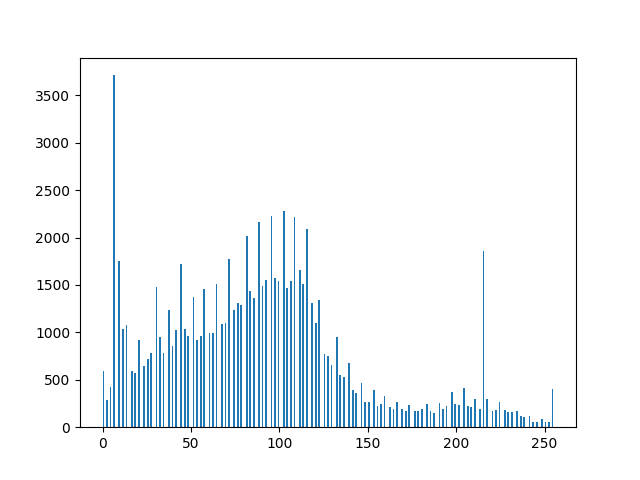
\includegraphics[width=1\textwidth]{../kids-stretched-histogram.png}
    \caption{Histogram of stretched image}
\end{figure}



\section{Gamma}
\stepcounter{subsection}
\subsection{Determining the Gamma of Your Computer Monitor}
\subsubsection{Image corresponding to matching gray level}
\begin{figure}[H]
    \centering
    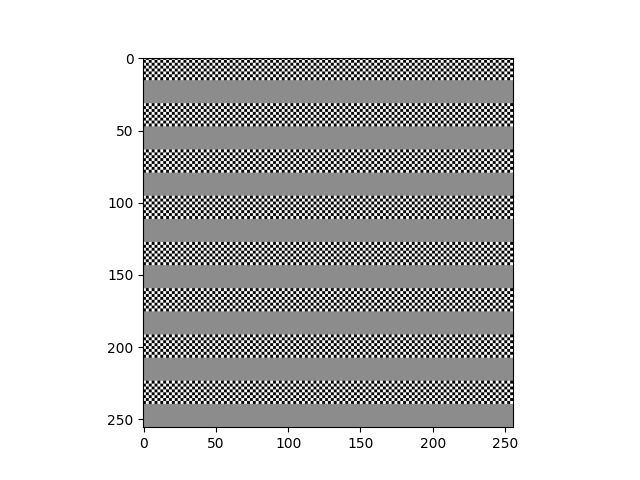
\includegraphics[width=1\textwidth]{../matching-gray-levels-140.png}
    \caption{Matching gray level}
\end{figure}
\subsubsection{Derivation of expression relating matching gray level to the value of $\gamma$}
By equating $I_c$ and $I_g$, we find

\begin{equation*}
    \frac{I_{255}}{2} = I_{255}(\frac{g}{255})^\gamma
\end{equation*}
\begin{equation*}
    \frac{1}{2} = (\frac{g}{255})^\gamma
\end{equation*}
\begin{equation*}
    \gamma = \log_{g/255}(\frac{1}{2})
\end{equation*}

\subsubsection{Measured gray level and mesured $\gamma$}
\begin{center}
    Measured gray level: 162

    Measured $\gamma$ value: 1.52785
\end{center}

\subsection{Gamma Correction}
\subsubsection{Original and corrected images}
\begin{figure}[H]
    \centering
    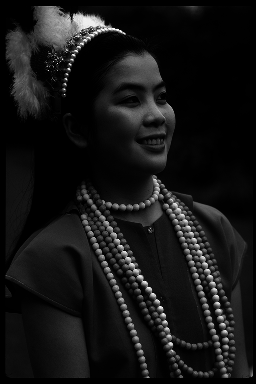
\includegraphics[width=0.5\textwidth]{../linear.png}
    \caption{Original version of linear.tif}
\end{figure}
\begin{figure}[H]
    \centering
    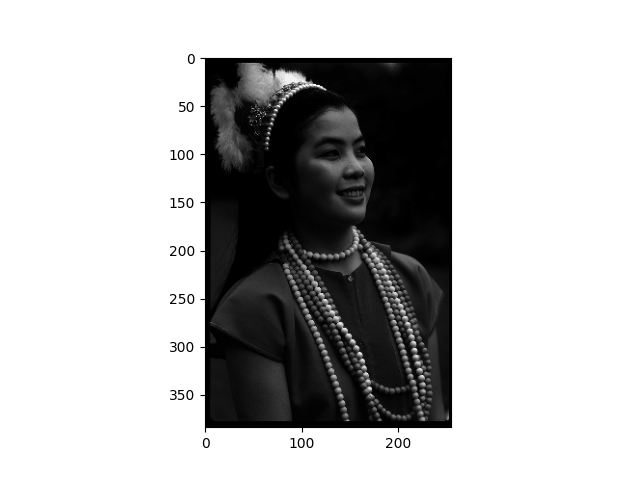
\includegraphics[width=1\textwidth]{../linear-gamma-corrected.png}
    \caption{Gamma-corrected version of linear.tif}
\end{figure}
\subsubsection{Formula used to transform the original image}
The below formula transforms pixels in the original image x to the gamma-corrected pixels y.
\begin{equation*}
    y = x^{1/\gamma}
\end{equation*}

\subsection{Second section of gamma correction}
\subsubsection{Corrected image}
\begin{figure}[H]
    \centering
    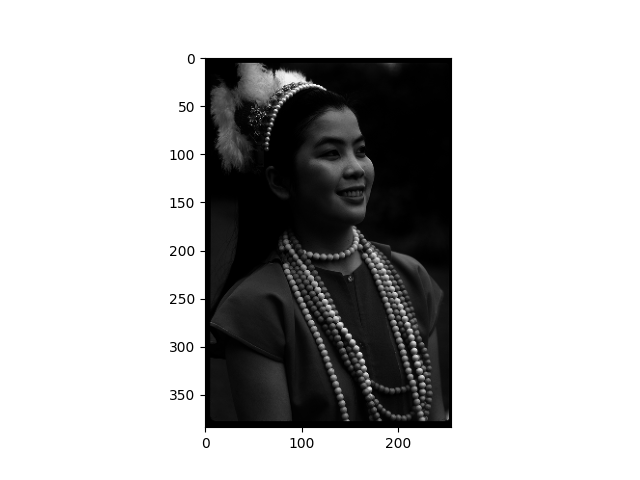
\includegraphics[width=1\textwidth]{../gamma15-gamma-corrected.png}
    \caption{Corrected version of gamma15.tif}
\end{figure}
\subsubsection{Procedure used to change the gamma correction of the original image}
The procedure is straightforward. First, undo the $\gamma = 1.5$ correction by raising each pixel value to the power of 1.5. Then just apply the same formula in section 4.3.2 with the value of $\gamma$ determined in section 4.2.3 above.



\end{document}
